\documentclass{standalone}
\usepackage{mathtools} % mathtools => amsmath
\usepackage{tikz} % pour \includegraphics
\usetikzlibrary{matrix,decorations.pathreplacing}

\def\rotation#1{\begin{smallmatrix}\cos(\alpha_{#1})&-\sin(\alpha_{#1})\\\sin(\alpha_{#1})&\phantom{-}\cos(\alpha_{#1})\end{smallmatrix}}

\begin{document}
  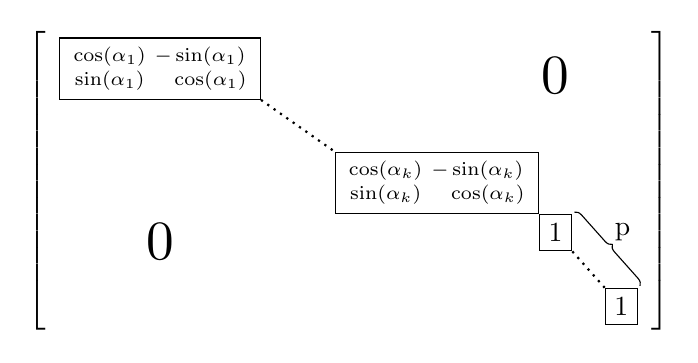
\begin{tikzpicture}
    \matrix[matrix of math nodes, left delimiter={[}, right delimiter={]},,nodes in empty cells] (M)
    {
      |[draw]|\rotation{1}&&&&&\\
      &\strut\hspace{7mm}&&&&\\
      &&|[draw]|\rotation{k}&&&\\
      &&&|[draw]|1&&\\
      &&&&\phantom{1}&\\
      &&&&&|[draw]|1\\
    };
    \draw[dotted,thick] (M-1-1.south east) -- (M-3-3.north west);
    \draw[dotted,thick] (M-4-4.south east) -- (M-6-6.north west);
    \draw[decorate,decoration={brace,raise=1pt}] (M-4-4.north east) -- node[above right]{p}(M-6-6.north east);
    \path (M-4-1) node[scale=2]{0};
    \path (M-1-4) node[scale=2]{0};
  \end{tikzpicture}
\end{document}
